\section{随机变量}

\subsection{基本概念}

\begin{definition}[随机变量]
随机变量是试验结果的实值函数。
\begin{figure}[H]
    \centering
    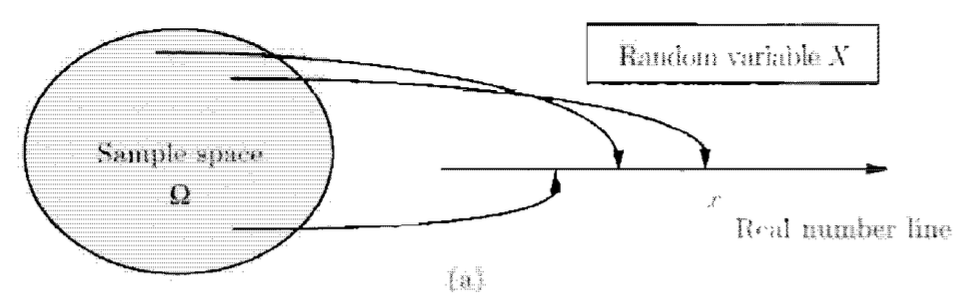
\includegraphics[width=0.65\linewidth]{figs/随机变量示意图.png}
    \caption{随机变量示意图}
    \label{fig:random-variable}
\end{figure}
\end{definition}
\begin{com}
一般用大写字母表示随机变量,小写字母表示其取值。
\end{com}

\begin{definition}[离散随机变量]
若一个随机变量的值域为有限集或可数集,则称这个随机变量是离散的。
\end{definition}

\begin{definition}[概率质量函数]
定义随机变量 $X$ 取值为 $x$ 的概率为事件 $\{X=x\}$ 的概率,即所有与 $x$ 对应的试验结果组成的事件的概率,记作 $p_X(x)$,即:
\[p_X(x)=\Pb(\{X=x\})\]
称 $p_X$ 为 $X$ 的概率质量函数 (PMF).
\end{definition}

\begin{property}
PMF 满足非负性和归一化条件:
\[\sum_x p_X(x)=\sum_x\Pb(X=x)=1\]
\end{property}
\begin{property}
设 $S$ 为任一 $X$ 可能取值的集合,则:
\[\Pb(X\in S)=\sum_{x\in S}p_X(x)\]
\end{property}

\begin{example}
常见的离散随机变量包括伯努利、二项、几何和泊松随机变量等,详见附录 \ref{sec:random-variables}.
\end{example}

\begin{definition}[连续随机变量,概率密度函数]
对随机变量 $X$,若存在一个非负函数 $f_X$,使得:
\[
\Pb(X\in B)=\int_Bf_X(x)\mathrm dx
\]
对实数轴的集合 $B$ 都成立\footnote{本书只考虑黎曼积分,且 $f_X$ 为有有限/可数个间断点的分段连续函数。},则称 $X$ 为连续的随机变量,函数 $f_X$ 称为概率密度函数 (PDF). 特别地,当 $B$ 是一个区间时,有:
\[
\Pb(a\leq X\leq b)=\int_a^bf_X(x)\mathrm dx
\]
\end{definition}
\begin{property}
PDF 满足非负性和归一化条件:
\[\int_{-\infty}^{\infty}f_X(x)\mathrm dx=\Pb(-\infty<X<\infty)=1\]
\end{property}
\begin{property}
对于充分小的 $\delta$,有:
\[\Pb(x\leq X\leq x+\delta)=\int_x^{x+\delta}f_X(x)\mathrm dx\approx f(x)\cdot\delta\]
\end{property}

\begin{example}
常见的连续随机变量包括均匀、指数和正态随机变量等,详见附录 \ref{sec:random-variables}.
\end{example}


\subsection{分布函数}

\begin{definition}[分布函数]
设 $X$ 是一个随机变量(离散或连续),定义其分布函数(CDF)$F_X$ 为:
\[
F_X(x)=\Pb(X\leq x)=\begin{dcases}
    \sum_{k\leq x}p_X(k),&\text{$X$ 离散}\\
    \int_{-\infty}^xf_X(t)\mathrm dt,&\text{$X$ 连续}
\end{dcases}
\]
\end{definition}
\begin{com}
分布函数统一刻画了离散和连续情形。离散情形下的 PMF、连续情形下的 PDF 和一般情形下的 CDF 都是相应随机变量的概率律。
\end{com}

\begin{property}
设 $F_X$ 是随机变量 $X$ 的分布函数,则:
\begin{itemize}
    \item $F_X$ 单调非减。
    \item $F_X(x)\to 0\;(x\to-\infty),;F_X(x)\to1(x\to\infty)$.
    \item 当 $X$ 是离散随机变量时,$F_X$ 是阶梯函数。
    \item 当 $X$ 是连续随机变量时,$F_X$ 是连续函数。
\end{itemize}
\end{property}

\begin{theorem}[分布列与分布函数]
设 $X$ 是离散随机变量且取整数值,则:
\[
F_X(k)=\sum_{i=-\infty}^kp_X(i),\quad p_X(k)=F_X(k)-F_X(k-1)
\]
\end{theorem}
\begin{theorem}[概率密度函数与分布函数]
设 $X$ 是连续随机变量,则:
\[
F_X(x)=\int_{-\infty}^xf_X(t)\mathrm dt,\quad f_X(x)=\frac{\mathrm d}{\mathrm dx}F_X(x)
\]
第二个等式只在分布函数可微处成立。
\end{theorem}


\subsection{期望和方差}

\begin{definition}[期望/均值]
随机变量 $X$ 的期望定义为:
\[
\E X=\begin{dcases}
    \sum_x xp_X(x),&\text{$X$ 离散}\\
    \int_{-\infty}^{\infty}xf_X(x)\mathrm dx,&\text{$X$ 连续}
\end{dcases}
\]
特别地,对于连续情形,若 $f_X$ 不是绝对可积的,即 $\int_{-\infty}^\infty |x|f_X(x)\mathrm dx=\infty$,则称期望不存在。
\end{definition}

\begin{definition}[矩,中心矩]
定义随机变量 $X$ 的 $n$ 阶矩为 $\E[X^n]$,$n$ 阶中心矩为 $\E[(X-\E X)^n]$.
\end{definition}

\begin{definition}[方差,标准差]
定义随机变量 $X$ 的方差为其 2 阶中心矩,标准差为方差的平方根:
\[
\var(X)=\E\left[(X-\E X)^2\right],\quad \sigma(X)=\sqrt{\var(X)}
\]
\end{definition}

\begin{theorem}[随机变量函数的期望]
设 $X$ 是一随机变量,则 $Y=g(X)$ 的期望为:
\[\E Y=\E[g(X)]=\begin{dcases}
    \sum_xg(x)p_X(x),&\text{$X$ 离散}\\
    \int_{-\infty}^{+\infty}g(x)f_X(x)\mathrm dx,&\text{$X$ 连续}
\end{dcases}
\]
因此,我们不必先求出 $Y$ 的分布,只需知道 $X$ 的分布就能求出 $Y$ 的期望。
\end{theorem}

\begin{theorem}[随机变量的线性函数的期望和方差]
设 $X$ 是一个随机变量,$Y=aX+b$,其中 $a,b$ 为常数,则:
\[\E Y=a\E X+b,\quad \var(Y)=a^2\var(X)\]
\end{theorem}
\begin{proof}
仅对离散情形证明,连续情形类似。
\begin{gather*}
\E Y=\sum_x(ax+b)p_X(x)=a\sum_x xp_X(x)+b\sum_xp_X(x)=a\E X+b\\
\var(Y)=\E[(Y-\E Y)^2]=\E[((aX+b)-(a\E X+b))^2]=a^2\E[(X-\E X)^2]=a^2\var(X)
\end{gather*}
\end{proof}

\begin{theorem}[用矩表达方差]
设 $X$ 是一个随机变量,则:
\[
\var(X)=\E[X^2]-(\E X)^2
\]
\end{theorem}
\begin{proof}
\begin{align*}
\var(X)&=\E\left[(X-\E X)^2\right]\\
&=\E\left[X^2-2X\E X+(\E X)^2\right]\\
&=\E[X^2]-2 \E X\cdot \E X+(\E X)^2\\
&=\E[X^2]-(\E X)^2
\end{align*}
\end{proof}

\begin{example}
常见随机变量的期望和方差及其推导过程见附录 \ref{sec:random-variables}.
\end{example}


\subsection{联合分布与边缘分布}

\begin{figure}[H]
    \centering
    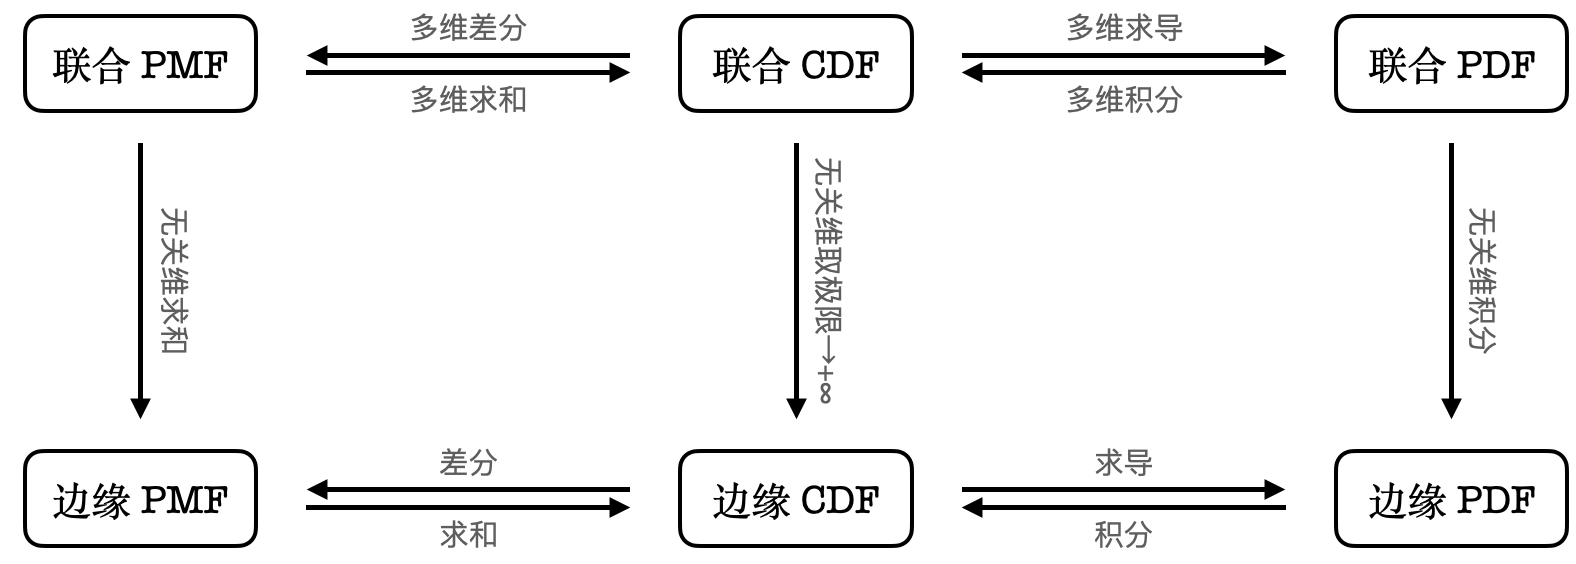
\includegraphics[width=0.8\linewidth]{figs/联合分布与边缘分布.png}
    \caption{联合分布与边缘分布的关系概览}
    \label{fig:union-marginal}
\end{figure}

\begin{definition}[联合概率质量函数]
设 $X,Y$ 是离散随机变量,定义 $(X,Y)$ 取值 $(x,y)$ 的概率为事件 $\{X=x,Y=y\}$ 的概率,记作 $p_{X,Y}(x,y)$,即:\[p_{X,Y}(x,y)=\Pb(X=x,Y=y)\]
称 $p_{X,Y}$ 为 $X,Y$ 的联合概率质量函数。
\end{definition}

\begin{definition}[联合概率密度函数]
设 $X,Y$ 是连续随机变量,若存在一个非负二元函数 $f_{X,Y}$ 使得:
\[
\Pb((X,Y)\in B)=\iint_{(x,y)\in B}f_{X,Y}(x,y)\mathrm dx\mathrm dy
\]
对平面上任意集合 $B$ 成立,则称 $f_{X,Y}$ 为联合概率密度函数。特别地,当 $B$ 是一个矩形区域时有:
\[
\Pb(a\leq X\leq b,c\leq Y\leq d)=\int_c^d\int_a^b f_{X,Y}(x,y)\mathrm dx\mathrm dy
\]
\end{definition}

\begin{property}
联合 PDF 满足归一化条件:
\[\int_{-\infty}^{\infty}\int_{-\infty}^{\infty}f_{X,Y}(x,y)\mathrm dx\mathrm dy=1\]
\end{property}
\begin{property}
对于充分小的 $\delta$,有:
\[\Pb(a\leq X\leq a+\delta,c\leq Y\leq c+\delta)=\int_c^{c+\delta}\int_a^{a+\delta}f_{X,Y}(x,y)\mathrm dx\mathrm dy\approx f_{X,Y}(a,c)\cdot\delta^2\]
\end{property}

\begin{theorem}[边缘概率质量函数]
设 $X,Y$ 是离散随机变量且联合 PMF 为 $p_{X,Y}$,则:
\[
p_X(x)=\sum_y p_{X,Y}(x,y),\quad p_Y(y)=\sum_xp_{X,Y}(x)
\]
称 $p_X$ 和 $p_Y$ 为边缘概率质量函数。
\end{theorem}

\begin{theorem}[边缘概率密度函数]
设 $X,Y$ 是连续随机变量且联合 PDF 为 $f_{X,Y}$,则:
\[
f_X(x)=\int_{-\infty}^{\infty}f_{X,Y}(x,y)\mathrm dy,\quad f_Y(y)=\int_{-\infty}^{\infty}p_{X,Y}(x)\mathrm dx
\]
称 $f_X$ 和 $f_Y$ 为边缘概率密度函数。
\end{theorem}

\begin{definition}[联合分布函数]
设 $X,Y$ 是两个随机变量(离散或连续),定义其联合分布函数为:
\[
F_{X,Y}(x,y)=\Pb(X\leq x,Y\leq y)
\]
\end{definition}

\begin{theorem}[联合概率密度函数与联合分布函数]
若随机变量 $X,Y$ 有联合概率密度函数 $f_{X,Y}$,则:
\[
F_{X,Y}(x,y)=\int_{-\infty}^x\int_{-\infty}^yf_{X,Y}(s,t)\mathrm ds\mathrm dt,\quad f_{X,Y}(x,y)=\frac{\partial^2}{\partial x\partial y}F_{X,Y}(x,y)
\]
\end{theorem}

\begin{theorem}[随机变量的二元函数的期望]
设 $X$ 和 $Y$ 是随机变量,则 $Z=g(X,Y)$ 的期望为:
\[
\E Z=\E[g(X,Y)]=\begin{dcases}
    \sum_{x}\sum_{y}g(x,y)p_{X,Y}(x,y),&\text{$X,Y$ 离散}\\
    \int_{-\infty}^{\infty}\int_{-\infty}^{\infty}g(x,y)f_{X,Y}(x,y)\mathrm dx\mathrm dy,&\text{$X,Y$ 连续}
\end{dcases}
\]
\end{theorem}

\begin{theorem}[随机变量的二元线性函数的期望]
设 $X$ 和 $Y$ 是随机变量,$a,b,c$ 为常数,则:
\[
\E[aX+bY+c]=a\E X+b\E Y+c
\]
\end{theorem}

\begin{theorem}[随机变量的多元线性函数的期望]
设 $X_1,X_2,\ldots,X_n$ 是 $n$ 个随机变量,$a_1,a_2,\ldots,a_n$ 是 $n$ 个常数,则:
\[
\E[a_1X_1+a_2X_2+\cdots+a_nX_n]=a_1\E X_2+a_2\E X_2+\cdots+a_n\E X_n
\]
\end{theorem}


\subsection{条件}

\begin{definition}[条件分布]
设 $X,Y$ 是离散随机变量,定义给定 $Y=y$ 下 $X$ 的条件概率质量函数为:
\[
p_{X\vert Y}(x\vert y)=\Pb(X=x\vert Y=y)=\frac{\Pb(X=x,Y=y)}{\Pb(Y=y)}=\frac{p_{X,Y}(x,y)}{p_Y(y)}
\]
类似地,设 $X,Y$ 是连续随机变量,定义给定 $Y=y$ 下 $X$ 的条件概率密度函数为:
\[
f_{X\vert Y}(x\vert y)=\frac{f_{X,Y}(x,y)}{f_Y(y)}
\]
\end{definition}

\begin{property}
条件 PMF/PDF 满足归一化条件:
\begin{gather*}
\sum_x p_{X\vert Y}(x\vert y)=1,\quad\text{$X$ 离散}\\
\int_{-\infty}^{\infty}f_{X\vert Y}(x\vert y)\mathrm dx=1,\quad\text{$X$ 连续}
\end{gather*}
\end{property}

\begin{theorem}[条件分布与联合分布]
设 $X,Y$ 是随机变量,由定义可知:
\begin{gather*}
p_{X,Y}(x,y)=p_Y(y)p_{X\vert Y}(x\vert y)=p_X(x)p_{Y\vert X}(y\vert x),\quad\text{$X$ 离散}\\
f_{X,Y}(x,y)=f_Y(y)f_{X\vert Y}(x\vert y)=f_X(x)f_{Y\vert X}(y\vert x),\quad\text{$X$ 连续}
\end{gather*}
\end{theorem}

\begin{theorem}[条件分布与边缘分布]
设 $X,Y$ 是随机变量,则根据全概率公式,有:
\begin{gather*}
p_X(x)=\sum_y p_{X\vert Y}(x\vert y)p_Y(y),\quad\text{$X$ 离散}\\
f_X(x)=\int_{-\infty}^{\infty} f_{X\vert Y}(x\vert y)f_Y(y)\mathrm dy,\quad\text{$X$ 连续}
\end{gather*}
\end{theorem}

\begin{theorem}[贝叶斯公式]
设 $X,Y$ 是随机变量,则有:
\begin{gather*}
p_{X\vert Y}(x\vert y)=\frac{p_{X,Y}(x,y)}{p_Y(y)}=\frac{p_{Y\vert X}(y\vert x)p_X(x)}{\sum_x p_{Y\vert X}(y\vert x)p_X(x)},\quad\text{$X,Y$ 离散}\\
f_{X\vert Y}(x\vert y)=\frac{f_{X,Y}(x,y)}{f_Y(y)}=\frac{f_{Y\vert X}(y\vert x)f_X(x)}{\int_{-\infty}^{\infty}f_{Y\vert X}(y\vert x)f_X(x)\mathrm dx},\quad\text{$X,Y$ 连续}
\end{gather*}
\end{theorem}

\begin{definition}[条件期望]
设 $X,Y$ 是随机变量,则给定 $Y=y$ 下 $X$ 的条件期望为:
\[
\E[X\vert Y=y]=\begin{dcases}
    \sum_xxp_{X\vert Y}(x\vert y),&\text{$X$ 离散}\\
    \int_{-\infty}^{\infty}xf_{X\vert Y}(x\vert y)\mathrm dx,&\text{$X$ 连续}
\end{dcases}
\]
对于随机变量的函数 $g(X)$,有:
\[
\E[g(X)\vert Y=y]=\begin{dcases}
    \sum_xg(x)p_{X\vert Y}(x\vert y),&\text{$X$ 离散}\\
    \int_{-\infty}^{\infty}g(x)f_{X\vert Y}(x\vert y)\mathrm dx,&\text{$X$ 连续}
\end{dcases}
\]
\end{definition}

\begin{note}
$\E[X|Y=y]$ 是一个数,其值依赖于 $y$,因此 $\E[X|Y]$ 是关于随机变量 $Y$ 的函数,从而也是一个随机变量。
\end{note}

\begin{theorem}[全期望公式]
设 $X,Y$ 是随机变量(离散或连续)且 $X$ 期望存在,则:
\[
\E X=\E[\E[X\vert Y]]=\begin{dcases}
    \sum_y \E[X\vert Y=y]p_Y(y),&\text{$Y$ 离散}\\
    \int_{-\infty}^{\infty} \E[X\vert Y=y]f_Y(y)\mathrm dy,&\text{$Y$ 连续}
\end{dcases}
\]
\end{theorem}
\begin{proof}
仅对离散情形证明,连续情形类似。
\begin{align*}
\E X&=\sum_x xp_X(x)\\
&=\sum_x x\sum_yp_{X|Y}(x\vert y)p_Y(y)\\
&=\sum_yp_Y(y)\sum_xxp_{X|Y}(x\vert y)\\
&=\sum_y \E[X\vert Y=y]p_Y(y)
\end{align*}
其中第二行应用了全概率公式。
\end{proof}

\begin{remark}
全期望公式常常是“反过来”使用的:当 $\mathbb EX$ 不好计算时,引入 $Y$ 转而计算 $\mathbb E[\mathbb E[X\vert Y]]$.
\end{remark}

\begin{definition}[条件方差]
设 $X,Y$ 是随机变量,则给定 $Y=y$ 下 $X$ 的条件方差为:
\[
\var(X\vert Y=y)=\E[(X-\E[X\vert Y=y])^2\vert Y=y]
\]
\end{definition}

\begin{note}
$\var(X\vert Y=y)$ 是一个数,其值依赖于 $y$,因此 $\var(X\vert Y)$ 是关于随机变量 $Y$ 的函数,从而也是一个随机变量,并且有:
\[
\var(X\vert Y)=\E[(X-\E[X\vert Y])^2\vert Y]=\E[X^2\vert Y]-(\E[X\vert Y])^2
\]
\end{note}

\begin{theorem}[全方差公式]
设 $X,Y$ 是随机变量且 $X$ 方差存在,则:
\[
\var(X)=\E[\var(X\vert Y)]+\var(\E[X\vert Y])
\]
\end{theorem}
\begin{proof}
\begin{align*}
\var(X)&=\E[X^2]-(\E X)^2\\
&=\E[\E[X^2\vert Y]]-(\E[\E[X\vert Y]])^2\\
&=\E[\E[X^2\vert Y]]-\E[(\E[X\vert Y])^2]+\E[(\E[X\vert Y])^2]-(\E[\E[X\vert Y]])^2\\
&=\E[\var(X\vert Y)]+\var(\E[X\vert Y])
\end{align*}
\end{proof}


\subsection{独立性}

\begin{definition}[独立]
设 $X,Y$ 是随机变量,称 $X$ 与 $Y$ 独立,若:
\begin{gather*}
p_{X,Y}(x,y)=p_X(x)p_Y(y),\quad\forall x,y,\quad\text{$X,Y$ 离散}\\
f_{X,Y}(x,y)=f_X(x)f_Y(y),\quad\forall x,y,\quad\text{$X,Y$ 连续}
\end{gather*}
\end{definition}
\begin{com}
离散情形下,若 $p_Y(y)>0$,则 $X$ 与 $Y$ 独立等价于:
\[p_{X\vert Y}(x\vert y)=p_X(x),\;\forall y\]
直观上,这说明 $Y$ 的取值不会给 $X$ 的取值带来信息。连续情形同理。
\end{com}

\begin{definition}[条件独立]
设 $X,Y,Z$ 是随机变量,给定 $Z=z$ 下(设 $p_Z(z)>0$ 或 $f_Z(z)>0$),称随机变量 $X$ 与 $Y$ 条件独立,若:
\begin{gather*}
p_{X,Y\vert Z}(x,y\vert z)=p_{X\vert Z}(x\vert z)p_{Y\vert Z}(y\vert z),\quad\forall x,y,\quad\text{$X,Y$ 离散}\\
f_{X,Y\vert Z}(x,y\vert z)=f_{X\vert Z}(x\vert z)f_{Y\vert Z}(y\vert z),\quad\forall x,y,\quad\text{$X,Y$ 连续}
\end{gather*}
\end{definition}

\begin{theorem}
若随机变量 $X,Y$ 相互独立,则:
\[
\E[XY]=\E X\E Y
\]
进一步地,对任意函数 $g,h$,有:
\[
\E[g(X)h(Y)]=\E[g(X)]\E[h(Y)]
\]
\end{theorem}
\begin{proof}
仅对离散情形证明,连续情形类似。
\begin{align*}
\E[XY]&=\sum_x\sum_y xyp_{X,Y}(x,y)\\
&=\sum_x\sum_y xyp_X(x)p_Y(y)\\
&=\sum_x xp_X(x)\sum_y yp_Y(y)\\
&=\E X\E Y
\end{align*}
第二个式子类似可证。
\end{proof}

\begin{corollary}
若随机变量 $X,Y$ 独立,则对任意函数 $g,h$,有 $g(X)$ 与 $h(Y)$ 独立。
\end{corollary}

\begin{theorem}
若随机变量 $X,Y$ 相互独立,则:
\[
\var(X+Y)=\var(X)+\var(Y)
\]
\end{theorem}
\begin{proof}
令 $\tilde X=X-\E X,\,\tilde Y=Y-\E Y$,由于方差在加减常数后保持不变,所以:
\begin{align*}
\var(X+Y)&=\var(\tilde X+\tilde Y)\\
&=\E[(\tilde X+\tilde Y)^2]\\
&=\E[{\tilde X}^2+2\tilde X\tilde Y+{\tilde Y}^2]\\
&=\E[{\tilde X}^2]+2\E[\tilde X\tilde Y]+\E[{\tilde Y}^2]\\
&=\var X+\var Y
\end{align*}
其中利用了 $\E[\tilde X\tilde Y]=\E[\tilde X]\E[\tilde Y]=0$.
\end{proof}

\begin{definition}[多个随机变量独立性]
称随机变量 $X,Y,Z$ 相互独立,若:
\begin{gather*}
p_{X,Y,Z}(x,y,z)=p_X(x)p_Y(y)p_Z(z),\quad\forall x,y,z,\quad\text{$X,Y,Z$ 离散}\\
f_{X,Y,Z}(x,y,z)=f_X(x)f_Y(y)f_Z(z),\quad\forall x,y,z,\quad\text{$X,Y,Z$ 连续}
\end{gather*}
\end{definition}

\begin{theorem}[多个独立随机变量和的方差]
设 $X_1,X_2,\ldots,X_n$ 为相互独立的随机变量,则:
\[
\var(X_1+X_2+\cdots+X_n)=\var(X_1)+\var(X_2)+\cdots+\var(X_n)
\]
\end{theorem}


% \subsection{正态随机变量}

% \begin{definition}[正态随机变量/高斯随机变量]
% 称连续随机变量 $X$ 为正态或高斯的,若其 PDF 为:
% \[
% f_X(x)=\frac{1}{\sqrt{2\pi}\sigma}e^{-\frac{(x-\mu)^2}{2\sigma^2}}
% \]
% 其中 $\mu,\sigma$ 是参数。
% \end{definition}

% \begin{theorem}[正态分布的均值和方差]
% 设 $X$ 为
% \end{theorem}
